\subparagraph{}
Just like for the question 1, we will transform this problem into a 2D linear optimization problem, so that we can use the (expected) linear runing-time 2D linear optimization algorithm already studied during the course.

\subparagraph{}
Let suppose that we have $n$ red points, of coordinates $(rx_i,ry_i) \forall i \in 1,..,n$ and $m$ green points of coordinates $(gx_i, gy_i) \forall i \in 1,..,m$. Our goal is to find a line separating the green points from the red points (we suppose that our computer is not affected by daltonism).

Generally speaking, the cartesian equation of a line is of the form $n_xx+n_yy=d$. It is very much like the equation of a plane in 3D: here $(n_x,n_y)$ is the "normal" of the line, and $d$ is the distance of the line to the origin.

However, the general equation of a line in 2D uses three parameters. To be able to use the 2D linear optimization algorithm, we would like to have only two parameters. In fact, we can use a parametric representation of a line with only two parameters to represent the lines that are not vertical (the lines for which $n_y \neq 0$).
Therefore, a non-vertical line can be represented by an equation of the form $y = n_1x+n_2$.

\subparagraph{}
Is it legit to restrict the line that we will find to a non-vertical line? Yes it is, because if a vertical line separates the red points from the green points, we can find a non-vertical line that will fit too: as we have a finite number of distinct points, we know that there is a guaranteed distance $\epsilon$ from one point to another one.
Moreover we know that three points are never aligned, therefore at most two points are on a line, the others are at least at a distance $\mu$ to the line: we can "tilt" the vertical line so that we have a non-vertical line separating the red points from the green points (as show the figure 1).

\graphicspath{./}
\begin{figure}[h]
	\caption{Tilting of a vertical line to a non-vertical one.}
    \centering
	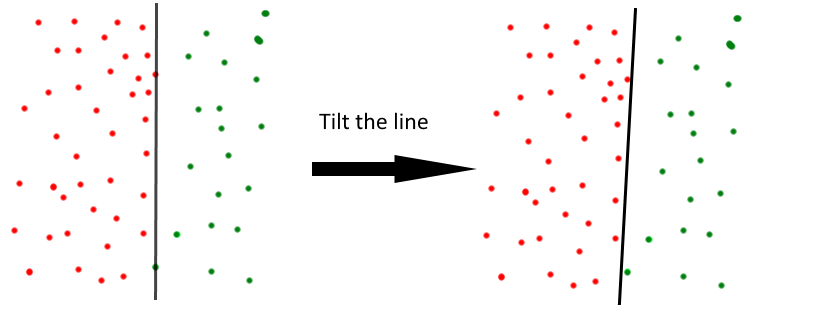
\includegraphics[height = 150px]{Tilted_line.png}
\end{figure}

Because of that, we will be searching a line represented by the equation $y = n_1x+n_2$ of parameters $(n_1,n_2)$.

\subparagraph{}
A point is said "under" a line of parameters $(n_1,n_2)$ if its coordinates $(x,y)$ verify $y \leq n_1x+n_2$, while it is considered "above" the line if we have $y \geq n_1x+n_2$.

This can be rewritten as $(-x)n_1 + (-1)n_2 \leq -y$ for "under", and $xn_1+n_2 \leq y$ for "above". Those are constraints for a 2D linear optimization problem!

Thus, we would like to specify our constraints like this: $(-rx_i)n_1 + (-1)n_2 \leq -ry_i \forall i \in 1,..,n$ for red points ("under") and $gx_in_1+n_2 \leq gy_i \forall i \in 1,..,m$ for green points ("above").
However, there are cases where we can not find a line such as the red poins are "under" and the green points "above", for example in the case presented by the following figure.

\graphicspath{./}
\begin{figure}[h]
	\caption{In this case, red points can not be under the line.}
	\centering
	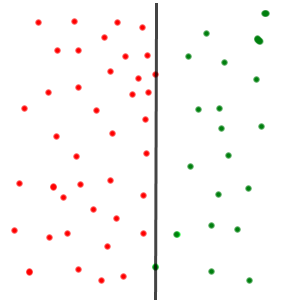
\includegraphics[height = 150px]{Red_points_never_under.png}
\end{figure}

In these cases we must run our optimization algorithm another time to check if we can find a line which separates the points in the other way, with the red points "above" and the green points "under" (reversing the constraints).

\subparagraph{}
As the function to optimize must be linear and there is no line better than another one, we will optimize the function $f(n_1,n_2)=0$.

\subparagraph{}
Therefore, we have reformulated the problem in terms of a 2D optimization problem, that we may try to solve two times (one time where we are searching for a line where the red points are "under"/green points "above", the other time where we search for a line where the red points "above"/green points "under").

Thanks to this reformulation of the problem we can claim that we have an $O(n+m)$ expected running time algorithm solving that problem: we use the 2D linear optimization algorithm as seen during the class where we incrementally find a solution satisfying more and more constraints, at least one time, at most two times.